\documentclass[english,serif,mathserif,usenames,dvipsnames]{beamer}
\usetheme[informal]{gc3}

\usepackage[T1]{fontenc}
\usepackage[utf8]{inputenc}
\usepackage{babel}

\usepackage{fancyvrb}
%% This is optional: it adds a few commands and environment we
%% regularly use in our slide sets
\usepackage{gc3}

\lstnewenvironment{stdout}{\lstset{language=sh,basicstyle=\tiny\ttfamily\bfseries}}{}%


\begin{document}

%% Optional Argument in [Brackets]: Short Title for Footline
\title[GC3Pie Tools]{An Introduction to GC3Pie Session-based scripts}
\author{Riccardo Murri \texttt{<riccardo.murri@gmail.com>}}
\date{\today}

%% Makes the title slide
\maketitle

% # Agenda (1/3)
%
% 1. Introduction
%    * What is GC3Pie?

\begin{frame}
  \frametitle{What is GC3Pie?}
  GC3Pie is \ldots
  \begin{enumerate}
  \item An \emph{opinionated} Python framework for defining and running computational workflows;
  \item \alert<2->{A \emph{rapid development toolkit} for running user applications on clusters and IaaS cloud resources;}
  \item The worst name ever given to a middleware piece\ldots
  \end{enumerate}

  \uncover<2->{As \emph{users}, you're mostly interested in this part.}
\end{frame}


\begin{frame}
  \frametitle{Who am I?}
  \begin{center}
    Systems administrator and programmer.
    \\ \+
    At UZH since 2010, first at GC3 then at S3IT.
    \\ \+
    Developer of GC3Pie since 2010.
  \end{center}
\end{frame}


\begin{frame}
  \begin{center}
    {\Huge and what about you?}
  \end{center}
\end{frame}


\begin{frame}
  \frametitle{Outline of this training, 1}
  \begin{enumerate}
  \item Concepts and glossary
  \item Usage of a session-based script
  \item Resubmission and dealing with errors
  \item Command-line tools mainly useful for debugging
  \end{enumerate}
\end{frame}


\begin{frame}
  \frametitle{Outline of this training, 2}
  \begin{center}
    We'd like the training to be \\ as interactive and informal as possible.

    \+ If you have a question, just ask -- don't wait.
  \end{center}
\end{frame}


% chapter division
\section{Concepts and glossary}
\part{Concepts and glossary}

% 2. Concepts and glossary
%    * Task / Application / Run

\begin{frame}
  \frametitle{GC3Pie glossary: Application}
  \begin{quote}
    GC3Pie runs \alert<2-3>{user applications}
    \\
    on clusters and IaaS cloud resources
  \end{quote}

  \uncover<2-3>{
    \+ \alert<2>{An \texttt{Application} is a just command to execute.}

    \+
    \only<2>{If you can run it in the terminal, \\ you can run it in GC3Pie.}
    \only<3>{
      \alert<3>{A single execution of an \texttt{Application} \\ is indeed called a \texttt{Run}.}

      \+ (Other systems might call this a ``Job''.)
    }
  }
\end{frame}



\begin{frame}
  \frametitle{GC3Pie glossary: Task}
  \begin{quote}
    GC3Pie \alert{runs} user applications
    \\
    on clusters and IaaS cloud resources
  \end{quote}

  \+ More generally, GC3Pie runs \texttt{Task}s.

  \+ \texttt{Task}s are a superset of applications,
  \\ in that they include workflows.

  \+ More on this later!
\end{frame}


%    * Resources
%      - _Introduce command `gservers` here? To start with a concrete step..._
\begin{frame}
  \frametitle{GC3Pie glossary: Resources}
  \begin{quote}
    GC3Pie runs user applications
    \\
    on \alert{clusters and IaaS cloud} resources
  \end{quote}

  \+ \alert{\texttt{Resource}s are the computing infrastructures \\ where GC3Pie executes applications.}

  \+ Resources include: your laptop, the ``Hydra'' cluster, the Science Cloud, Amazon AWS.
\end{frame}


\begin{frame}[fragile]
  \frametitle{The \texttt{gservers} command}

  The \texttt{gservers} command is used to see \alert<2>{configured} and
  available resources.

\+
\begin{stdout}
> gservers
+---------------------+--------------------------+-----------+
|                     | localhost                |           |
+---------------------+--------------------------+-----------+
|            frontend | ( Frontend host name )   | localhost |
|                type | ( Access mode )          | shellcmd  |
|             updated | ( Accessible? )          | True      |
|              queued | ( Total queued jobs )    | 0         |
|         user_queued | ( Own queued jobs )      | 0         |
|            user_run | ( Own running jobs )     | 6         |
|   max_cores_per_job | ( Max cores per job )    | 4         |
| max_memory_per_core | ( Max memory per core )  | 8GiB      |
|        max_walltime | ( Max walltime per job ) | 8hour     |
+---------------------+--------------------------+-----------+
\end{stdout}

\uncover<2>{\small \alert<2>{Resources are defined in file \texttt{\$HOME/.gc3/gc3pie.conf}}}
\end{frame}


\begin{frame}
  \frametitle{Warholize!}

\begin{semiverbatim}
    > ./warholize.py uzh-logo.png -C 1
\end{semiverbatim}

  \begin{tabular}[c]{ccc}
    
\includegraphics[width=0.4\textwidth]{uzh-logo.png}
    &
    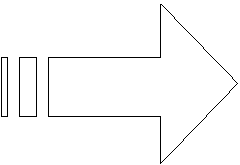
\includegraphics[width=0.1\textwidth]{arrow.pdf}
    &
    
\includegraphics[width=0.4\textwidth]{warholized-uzh-logo.png}
  \end{tabular}
\end{frame}


\begin{frame}
  \frametitle{Session-based scripts}

  \texttt{warholize.py} is a typical \emph{session-based script}.

  \+ A \emph{session} is just a named collection of jobs.

  \+ A \emph{session-based script} creates a session and runs all the
  jobs in it until completion.
\end{frame}


\begin{frame}
  \frametitle{Create a session}

  A session-based script \alert{creates a session}
  \\
  and runs all the jobs in it until completion.

  \+ Create session \texttt{logo-session}:
\begin{semiverbatim}
    > ./warholize.py uzh-logo.png -s logo-session
\end{semiverbatim}
\end{frame}


\begin{frame}
  \frametitle{Run a session to end}

  A session-based script creates a session
  \\
  and \alert{runs all the jobs in it until completion.}

  \+ Run jobs in session \texttt{logo-session},
  polling for updates every 5 seconds:
\begin{semiverbatim}
    > ./warholize.py -s logo-session -{}-watch 5
\end{semiverbatim}

  \+ \uncover<2>{
    You can stop a GC3Pie script by pressing \emph{Ctrl+C}.
    Run it again to resume activity from where it stopped.
  }
\end{frame}


\begin{frame}
  \frametitle{Alternate display of session contents}

  Display top-level tasks in session \texttt{logo-session}:
\begin{semiverbatim}
    > gsession list logo-session
\end{semiverbatim}
\end{frame}


\begin{frame}
  \frametitle{Alternate display of session contents}

  Display \emph{all} tasks in session \texttt{logo-session}:
\begin{semiverbatim}
    > gsession list --recursive logo-session
\end{semiverbatim}
\end{frame}


\begin{frame}
  \frametitle{Alternate display of session contents}

  Display summary of tasks in session \texttt{logo-session}:
\begin{semiverbatim}
    > gstat -n -b -s logo-session
\end{semiverbatim}
\end{frame}


\begin{frame}
  \frametitle{Display session history}

  Show log of activity on tasks in session \texttt{logo-session}:
\begin{semiverbatim}
    > gsession log logo-session
\end{semiverbatim}
\end{frame}


\begin{frame}
  \frametitle{Select execution resource}

  Select where applications will be run with option \texttt{-r}:
\begin{semiverbatim}
    > ./warholize.py -s logo-session -r localhost
\end{semiverbatim}

  \+ The resource name must exists in the configuration file (i.e.,
  check \texttt{gservers}' output).

  \+ Stopping a script and re-starting it with a different resource
  will likely result in an error: old tasks can no longer be found.
\end{frame}


%    * Session / Session-based script
%    * Workflows?
% 3. Use of a session-based script to run tasks
%    * Demo of the "Warholize" script
%    * Continuous execution (option `-C`)
%      - Inspect a session's contents while running:
%        * the `gstat` command
%        * `gsession log`
%        * `gtail` _(Ma anche no: non sono sicuro che funzioni ancora!)_
%    * Limit nr. of concurrently-running jobs (option `-J`)
%    * Select execution resource (option `-r`)
%    * Starting over (option `-N`)
%      - Alternatives:
%        * `gsession abort`
%        * `gkill`
% 4. Resubmission and dealing with errors
%    * `gselect`: Task selection
%    * `gresub`: Resubmission
%      - Hands-on: use `gselect` + `gresub` to resubmit failed tasks
% 5. Other command-line tools
%    * `ginfo`: Advanced task inspection
%      - Hands-on: how much memory did my job actually use?
%    * `gcloud`: Cloud backend management



\appendix
\part{Further reading}

\begin{frame}
How do we ``warholize'' an arbitrary image?

\+
\begin{enumerate}
\item Convert the original image to grayscale.
\item Colorize the grayscale image using three different colors for each tile.
\item Arrange all the colorized images into an $N\times N$ frame.
\end{enumerate}

\+
\begin{references}
  \url{http://gc3pie.googlecode.com/svn/trunk/gc3pie/docs/html/gc3libs/tutorial/warholize.html}
\end{references}
\end{frame}


\begin{frame}
  \frametitle{GC3Pie glossary: Task Collections}

  The basic unit of work in a GC3Pie workflow is called a \texttt{Task}.

  \+
  The \texttt{Application} class that you already know is a kind of
  \texttt{Task} (in programming speak, it's a derived class).

  \+
  A set of \texttt{Task}s is itself a \texttt{Task}, and is called a \texttt{TaskCollection}.
\end{frame}


\section{The End}
\begin{frame}[fragile]
  \frametitle{You have seen\ldots}
  \tableofcontents[sectionstyle=show/shaded]
\end{frame}

\end{document}

%%% Local Variables:
%%% mode: latex
%%% TeX-master: t
%%% End:
